Podemos crear algoritmos aún más potentes combinando un barrido de línea con un algoritmo de divide y vencerás. Un ejemplo es calcular el árbol de expansión mínimo de un conjunto de puntos, donde la distancia entre cualquier par de puntos es la distancia de Manhattan. Este es esencialmente el algoritmo presentado por Guibas y Stolfi.

Primero desglosamos esto en un problema más simple. Los algoritmos de árbol de expasión minima(\emph{MST}) estándar para grafos generales (p. ej., el algoritmo de Prim) pueden calcular el MST en tiempo O ($(E + N)\log N$) para aristas E. Si podemos explotar las propiedades geométricas para reducir el número de aristas a O($N$), entonces esto es simplemente O($N \log N$). De hecho, podemos considerar, para cada punto P, solo sus vecinos más cercanos en cada uno de los 8 octantes del plano (ver la figura a continuación). La figura muestra la situación en uno solo de los octantes, el Oeste-Noroeste. $Q$ es el vecino más cercano (con la línea discontinua que indica puntos a la misma distancia de Manhattan que $Q$), y $R$ es algún otro punto en el octante. Si $PR$ es una arista en un árbol de expansión, entonces puede eliminarse y reemplazarse por $PQ$ o $QR$ para producir un árbol de expansión mejor, porque la forma del octante garantiza que $|QR| = |PR|$. Por lo tanto, no necesitamos considerar $PR$ cuando construimos el árbol de expansión.

% TODO: \usepackage{graphicx} required
\begin{figure}[!h]
	\centering
	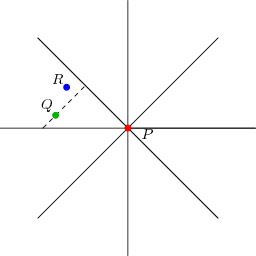
\includegraphics[width=0.25\linewidth]{img/octants}
	\label{fig:octants}
\end{figure}

Esto reduce el problema a encontrar el vecino más cercano en cada octante. Solo consideraremos el octante que se muestra; los otros no son diferentes y pueden manejarse por simetría. Debería quedar claro que dentro de este octante, encontrar el vecino más cercano es equivalente a simplemente encontrar el punto con el mayor valor de $x - y$, sujeto a un límite superior en $x + y$ y un límite inferior en $y$, y esta es la forma en el que consideraremos el problema.

Ahora imagine por el momento que el límite inferior de y no existe. En este caso podríamos resolver el problema para cada $P$ con bastante facilidad: barrer los puntos en orden creciente de $x + y$, y $Q$ será el punto con el mayor valor de $x - y$ de los vistos hasta ahora. Aquí es donde entra en juego el principio de divide y vencerás: dividimos el conjunto de puntos en dos mitades con una línea horizontal y resolvemos recursivamente el problema para cada mitad. Para los puntos $P$ en la mitad superior, no se necesita hacer nada más, porque los puntos en la mitad inferior no pueden jugar $Q$ con su $P$. Para la mitad inferior, debemos considerar que al ignorar la mitad superior hasta ahora, es posible que nos hayamos perdido algunos puntos más cercanos. Sin embargo, podemos tener en cuenta estos puntos de una manera similar a la anterior: recorrer todos los puntos en el orden $x + y$, siguiendo el mejor punto en la mitad superior (mayor valor $x - y$), y para cada punto en la mitad inferior, comprobando si este mejor punto de la mitad superior es mejor que el vecino actual.

Hasta ahora, he asumido alegremente que cualquier conjunto de puntos se puede dividir de manera eficiente en Y y también caminar en el orden $x + y$ sin decir cómo se debe hacer esto. De hecho, uno de los aspectos más hermosos de esta clase de algoritmos de divide y vencerás más barrido de línea es que tiene esencialmente la misma estructura que una ordenación por combinación, hasta el punto de que una ordenación por combinación $x + y$ puede ser doblado en el algoritmo de tal manera que cada subconjunto se ordena en $x + y$ justo cuando es necesario (los puntos inicialmente se ordenan en $Y$). Esto le da al algoritmo un tiempo de ejecución de O($N log N$).

La idea de encontrar el punto más cercano dentro de un rango de ángulo también se puede utilizar para resolver el problema euclidiano MST, pero el tiempo de ejecución O($N\log N$) ya no está garantizado en el peor de los casos, porque la distancia ya no es una ecuación lineal. En realidad, es posible calcular la MST euclidiana en tiempo O($N \log N$), porque es un subconjunto de la triangulación de Delaunay.
